\documentclass[hidelinks]{article}
\usepackage{fontawesome}
\usepackage{tabto} %tabCommand

\usepackage{titlesec}
\usepackage[utf8]{inputenc}
\usepackage{titling}
\usepackage{xcolor}
\usepackage{color}
\usepackage{smartdiagram}
\usepackage[margin=0.6in]{geometry}
\usepackage{hyperref}
\usepackage{tikz}
\usetikzlibrary{calc,positioning,backgrounds,matrix}
\usepackage[openbib]{currvita}
\usepackage[absolute]{textpos}
\usepackage{xhfill}\usepackage{amssymb} %checkbox
\usepackage{tikz}
\usetikzlibrary{trees}


\definecolor{dimgray}{rgb}{0.41, 0.41, 0.41}
\definecolor{blue}{RGB}{0,51,128}

% Title name
\renewcommand{\maketitle}{
\begin{center}
\Huge\bfseries
\color{dimgray}\thetitle
\vspace{0em}
\Large\bfseries
\vspace{0em}
\color{blue}\theauthor
{}
\end{center}
\vspace{-1em}
\xhrulefill{dimgray}{3pt}

}

\usepackage{sectsty}
\sectionfont{\color{blue}}
\renewcommand{\thesubsection}{}

\titleformat{\section}
{\Large\bfseries\uppercase}
{}
{-1em} 
{}
\titleformat{\subsection}
{\normalsize\bfseries}
{}
{0em} 
{}

\titleformat{\subsubsection}
{\normalsize\itshape}
{}
{0em} 
{}

 \smartdiagramset{
      bubble center node font = \small,
      bubble node font = \scriptsize,
      bubble center node size =2cm,
      bubble node size =2cm,
    }
\color{black}

\begin{document}
%\begin{textblock}{width}[xt,yt](X,Y)
\begin{textblock}{3}(.7,.25)
\section*{Birth Date}
15 July 1997
\section*{Address}
10 St. Ibrahim Baher Zaghlol, Manial, Cairo, Egypt
\section*{Mobile Number}
+201151280909
\section*{Mail}
\href{mailto: habiba.hamad97@eng-st.cu.edu.eg
}{\textbf{habiba.hamad97@eng-st.cu.edu.eg}}
\section*{Work Profiles}
\href{https://github.com/habiba1997}{github.com/habiba1997} \\*
\href{https://www.linkedin.com/in/habiba-ahmed-563399127}{linkedin.com/habiba-ahmed-563399127} \\*
\href{https://www.hackerrank.com/habiba_hamad97}{hackerrank.com/habiba\_hamad97}
\section*{Programistic Skills}
    \smartdiagram[bubble diagram]{\\ \\Java\\ \\,C++,Python,C\# , Algorithms \& \\Data Structure\\,Arduino,Latex, Object Oriented \\ Programing\\OOP}
    
\tikzstyle{every node}=[draw=blue,thin,anchor=west,blue]

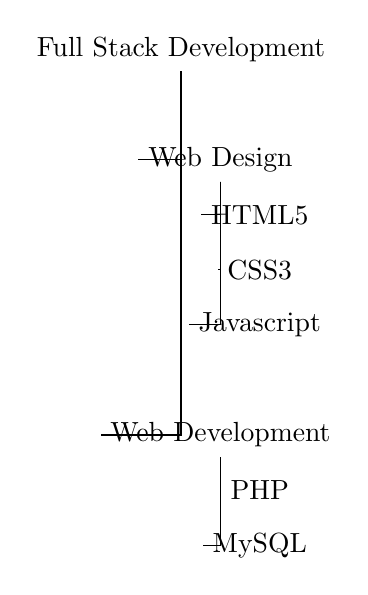
\begin{tikzpicture}[%
  grow via three points={one child at (0.5,-0.7) and
  two children at (0.5,-0.7) and (0.5,-1.4)},
  edge from parent path={(\tikzparentnode.south) |- (\tikzchildnode.west)}]
  \node {Full Stack Development}
          child [missing] {}		
    child { node {Web Design}
      child { node {HTML5}}
      child { node {CSS3}}
      child { node {Javascript}}
    }
       child [missing] {}				
    child [missing] {}				
    child [missing] {}
        child [missing] {}		
 child { node {Web Development}
      child { node {PHP}}
      child { node {MySQL}}
    }
    ;
\end{tikzpicture}
\end{textblock}

\begin{textblock}{9}(6,.1)

\title{Habiba Ahmed\\}
\author{System and Biomedical Engineering Student}
\maketitle
\vspace{-.75em}

\section*{Education}

\begin{cvlist}{}
\item[2015--2020] Systems and Biomedical Engineering, Cairo University \\* (GPA: 3.78)
\item[2013--2015] Oruba International High School (American Diploma)
\end{cvlist}

\section*{Competitions} 
\begin{cvlist}{}
\item[1/08/2018 -- 14/10/2018] Hospital System Innovation Competition, Cairo University Faculty of Engineering
\item[19/10/2018 -- 20/10/2018] IEEEXtreme Programming Competition

\end{cvlist}

\section*{Experience} 
\begin{cvlist}{}
\item[08/2018--Present] Media Member @ ESL\\Embedded System Laboratory
\item[08/2018--09/2018] Biomedical Machines Trainee @ Al Qasr Al Ayni
\item[07/2017--06/2018] Vice President @ Hand In Hand \\ Charity Student Activity
\item[09/2017--05/2018] Head Public Relation @ BEAT \\ Biomedical Engineering Awareness and Technology
\item[06/2017--09/2017] Fundrasing Member @ International Student Conference
\item[2017] Organizing Member @ The 2nd Biomedical Engineering Careers in the Egyptian Market Conference
\item[2016--2017]  Mechanic Representative for 1st year of Biomedical Engineering Batch, Cairo University
\item[02/2017--09/2017]Relation Member @ BEAT
\item[09/2016--06/2017]Logistics and Decoration Member @ Energia Powered\\Educational Student Activity

\end{cvlist}

\section*{Personal Projects}
\subsection{HNA hospital (Competition Project)}
A smart registration, data access and storage hospital system 

\subsection{Medium (Web Development Project)}
A simulation for medium.com website

\subsection{Immature Babies Nursery}
A baby incubator simulation using arduino, Color Sensor, Thermistor, and Turbine Flow Sensor

\subsection{Question and Answer Game}
A python GUI game where a player answer various questions related to his choosen subject



\end{textblock}
~\newpage
%That sounds exactly the problem  \null\newpage or (equivalently) \hbox{}\newpage should work, too.
%------------------------------------------------------------------
%------------------------------------------------------------------
%--------------new page-----------
%------------------------------------------------------------------
%------------------------------------------------------------------
\begin{textblock}{3}(.7,.25)
\section*{Interpersonal Skills}
%\includegraphics[scale=0.2]{Pie.png}
\makebox[0pt][l]\tab{\tab\color{blue}\hspace{0.1em}$\checkmark$}	Leadership 

\makebox[0pt][l]\tab{\color{blue}\hspace{0.1em}$\checkmark$}	Positive attitude

\makebox[0pt][l]\tab{\color{blue}\hspace{0.1em}$\checkmark$}	Time Management 

\makebox[0pt][l]\tab{\color{blue}\hspace{0.1em}$\checkmark$}	Assiduous 

\makebox[0pt][l]\tab{\color{blue}\hspace{0.1em}$\checkmark$}	Organized

\makebox[0pt][l]\tab{\color{blue}\hspace{0.1em}$\checkmark$}	Comunicative
     
\makebox[0pt][l]\tab{\color{blue}\hspace{0.1em}$\checkmark$}	Hardworker
 
\makebox[0pt][l]\tab{\color{blue}\hspace{0.1em}$\checkmark$}	Team Management 
 
\makebox[0pt][l]\tab{\color{blue}\hspace{0.1em}$\checkmark$}	Strong work ethics
 
\makebox[0pt][l]\tab{\color{blue}\hspace{0.1em}$\checkmark$}	Disciplined 
   
    

\section*{Languages}
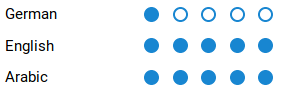
\includegraphics[scale=0.6]{language.png}
 
\section*{Interests}
Solving Codes, Web Development, Basketball \& Reading


\end{textblock}

\begin{textblock}{9}(6,.1)

\subsection{Blood Transfusion Warmer}
A blood IV tubing simulation using arduino, : Thermistor, and Heater

\subsection{Tooth Abscess Detection}
A tooth abcess detection project using arduino, Tilt, Photo-diode, Photo-resistor(LDR) and Photo-transistor
\section*{Certifications}
\begin{cvlist}{}
\item[9/2018--Present] Blockchain Intro \\ Certification authority IBM
\item[9/2018--Present] Cloud Intro \\ Certification authority IBM
\item[4/2017--Present] Work Smarter, Not Harder: Time Management for Personal \& Professional Productivity\\Certification authority Coursera
\item[2/2017--Present] Project Management: The Basics for Success\\Certification authority Coursera

\end{cvlist}


    
  
\end{textblock}




\end{document}

